\documentclass[sigconf]{acmart}
\settopmatter{printacmref=false, printccs=false, printfolios=true}
\renewcommand\footnotetextcopyrightpermission[1]{}

\usepackage{booktabs} % For formal tables

\begin{document}
\title{Iterative Histogram Equalization}

\author{Pedro Banha}
\email{pmt.lopes@campus.fct.unl.pt}

\author{Martin Magdalinchev}
\email{m.magdalinchev@campus.fct.unl.pt}

\maketitle

\section{Overview}
To develop this project, we analysed the given files and started by creating new file for each architectural version. This way, we can separately run and test each one of the versions. 
\section{Project Architecture}

\subsection{Code Architecture}
Our source code (project-57514-58172/src) is composed by the following files:

\subsubsection{main.cpp}
Main file that runs all possible tests, depending on which configuration is running.

\subsubsection{histogram\textunderscore eq.cpp}
Initial code for iterative histogram equalization (Sequential version)

\subsubsection{histogram\textunderscore par\textunderscore initial.cpp}
First parallel version of the sequential code

\subsubsection{histogram\textunderscore par\textunderscore second.cpp}
Second parallel version (improvements made over the initial parallel version)

\subsubsection{histogram\textunderscore par.cpp}
Final parallel version (improvements made over the second parallel version)

\subsubsection{histogram\textunderscore cuda.cu}
GPU-accelerated version of the final parallel version of the code

\subsubsection{dataset\textunderscore generator.cpp}
File that generates random images with given height and width

\subsection{CMakeLists.txt configuration}
To be able to run the tests, for each version of the code we added a configuration to create an executable with the main.cpp and the respective verion's histogram file. When the project is built, 6 executable are created for testing the solution:

\subsubsection{project}
Executable that runs the sequential version.

\subsubsection{project\textunderscore par}
Executable that runs the final parallelized version.

\subsubsection{project\textunderscore par\textunderscore initial}
Executable that runs the initial parallelized version.

\subsubsection{project\textunderscore par\textunderscore second}
Executable that runs the second parallelized version.

\subsubsection{project\textunderscore cuda}
Executable that runs the GPU-accelerated version off the final parallelized version.

\subsubsection{dataset\textunderscore generator}
Executable that runs the image generator

\subsection{Build instructions}
To build correctly the project, follow the following steps:
\begin{itemize}
    \item Clone the repository
    \item Navigate to project-57514-58172 folder
    \item Remove the existing build package(if any): rm -rf build
    \item Create build folder:mkdir build
    \item Run: sudo cmake -B build -S. (Note: use CUDACCXX=/usr/loccal/ccuda-11.8/bin/nvcc to specify the nvcc if needed)
    \item Then: cd build and finally: make
\end{itemize}

\subsection{Test instructions}
To execute manual test, run the command .\/{executable\textunderscore name} input\textunderscore image number\textunderscore iterations output\textunderscore image. 
In the project-57514-58172/scripts folder is a run\textunderscore tests.sh file, which runs all versions, for three different images(3000x2500px, 5184x3456px and 800x600px respectively). The output is written to the analysis.txt file in the same folder.
\section{Stage 1}
\subsection{Initial Parallelization}
The base file for this version is the sequential version of the code.
\subsubsection{Implementation}
After analyzing the sequential version, our first step was to refactor the code, more specifically the histogram\textunderscore equalization function, in order to split the parallelizable loops into their own functions. For each parallelized function, the basic "\# pragma omp parallel for" was used, except for the find\textunderscore cdf\textunderscore min, where "\#pragma omp parallel for reduction(min : cdf\textunderscore min)" was used. Additionally, the convert\textunderscore to\textunderscore grayscale function was improved (the two for loops were joined into one for loop for the combined sizes).
\subsubsection{Performance analysis}
\begin{figure}[h]
    \centering
    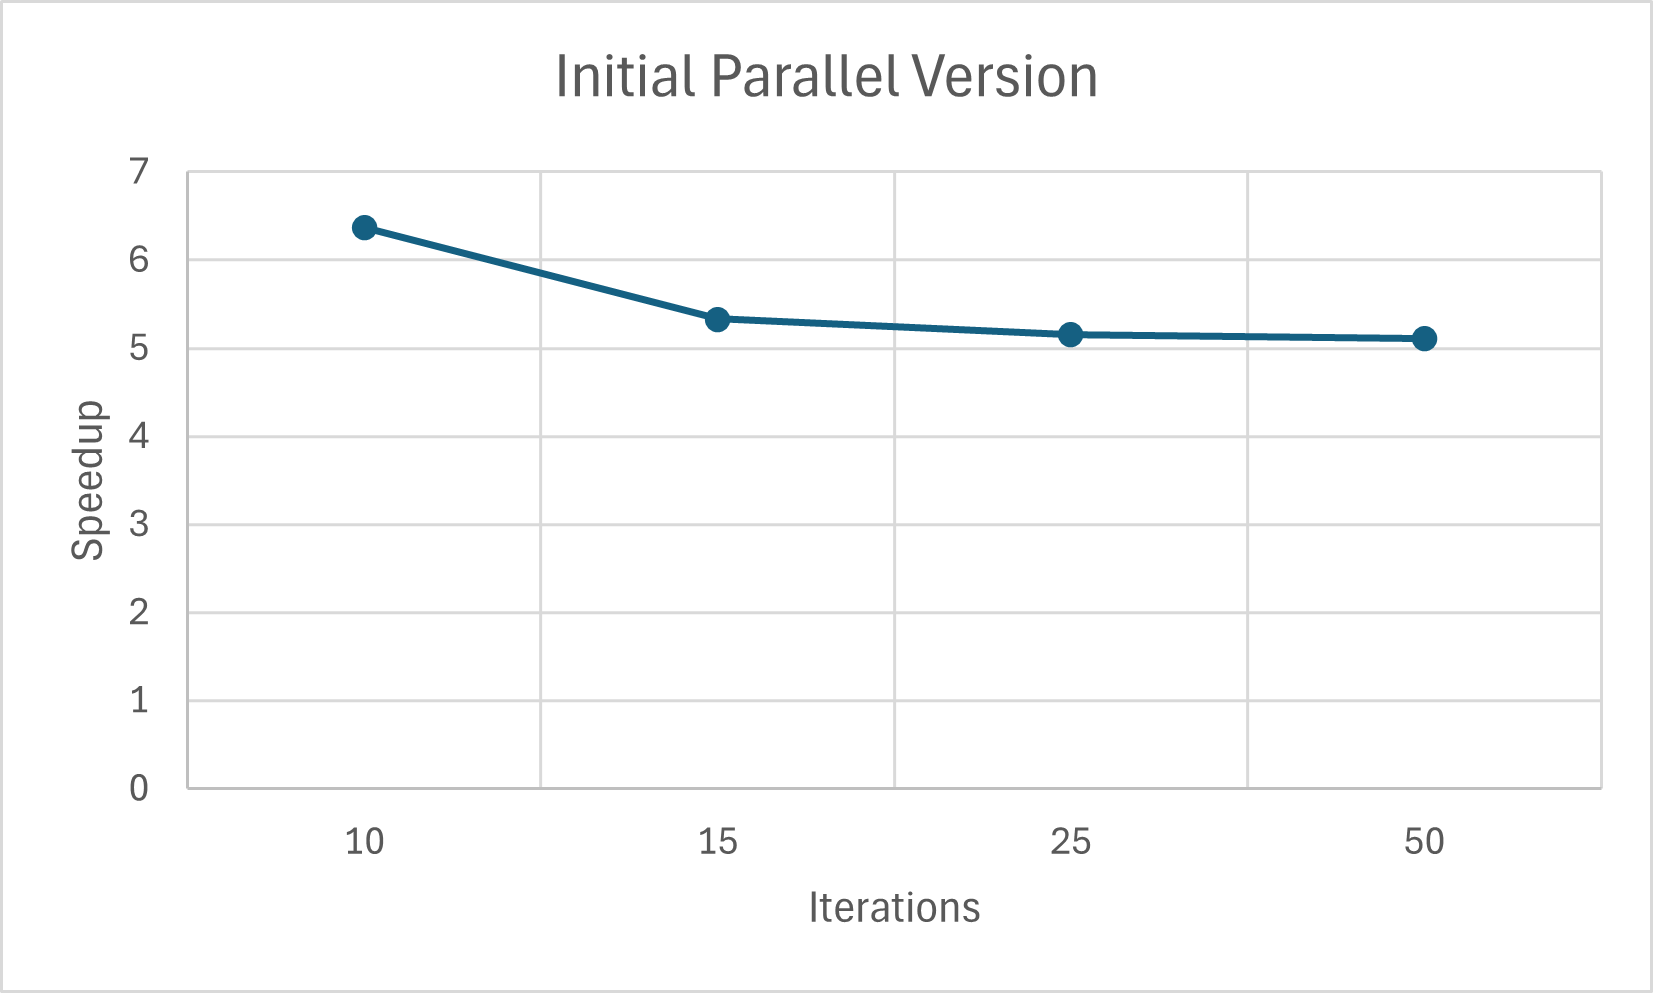
\includegraphics[width=0.5\textwidth]{InitialParallelSpeedup.png}
    \caption{Speedup of the Initial Parallel Version}
\end{figure}
After refactoring the code, we run different tests, with images with different sizes and different number of iterations. These were the results of the speedup between the sequential and this version, for an image of size 3000x2500 px:



As we can see, this initial change improved the efficiency of the solution, resulting in a Speedup of around 5.
\subsubsection{Profiler Analysis}
We also run the profiler in CLion for the sequential version and this first parallel implementation. We can observe that the existing hotspot in the histogram\textunderscore equalization function was mitigated. 
\begin{figure}[h]
    \centering
    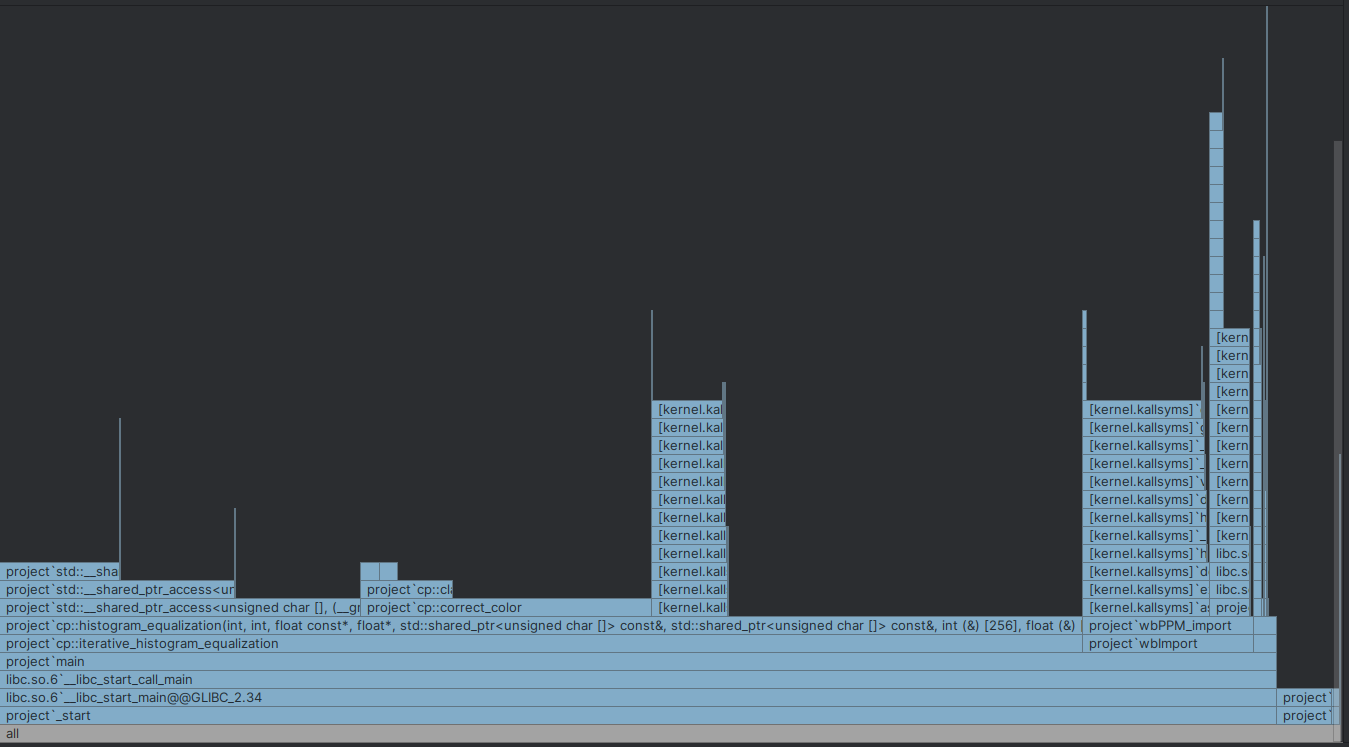
\includegraphics[width=0.5\textwidth]{SequentialProfiler.png}
    \caption{CLion Profiler of the Sequential Version}
\end{figure}
\begin{figure}[h]
    \centering
    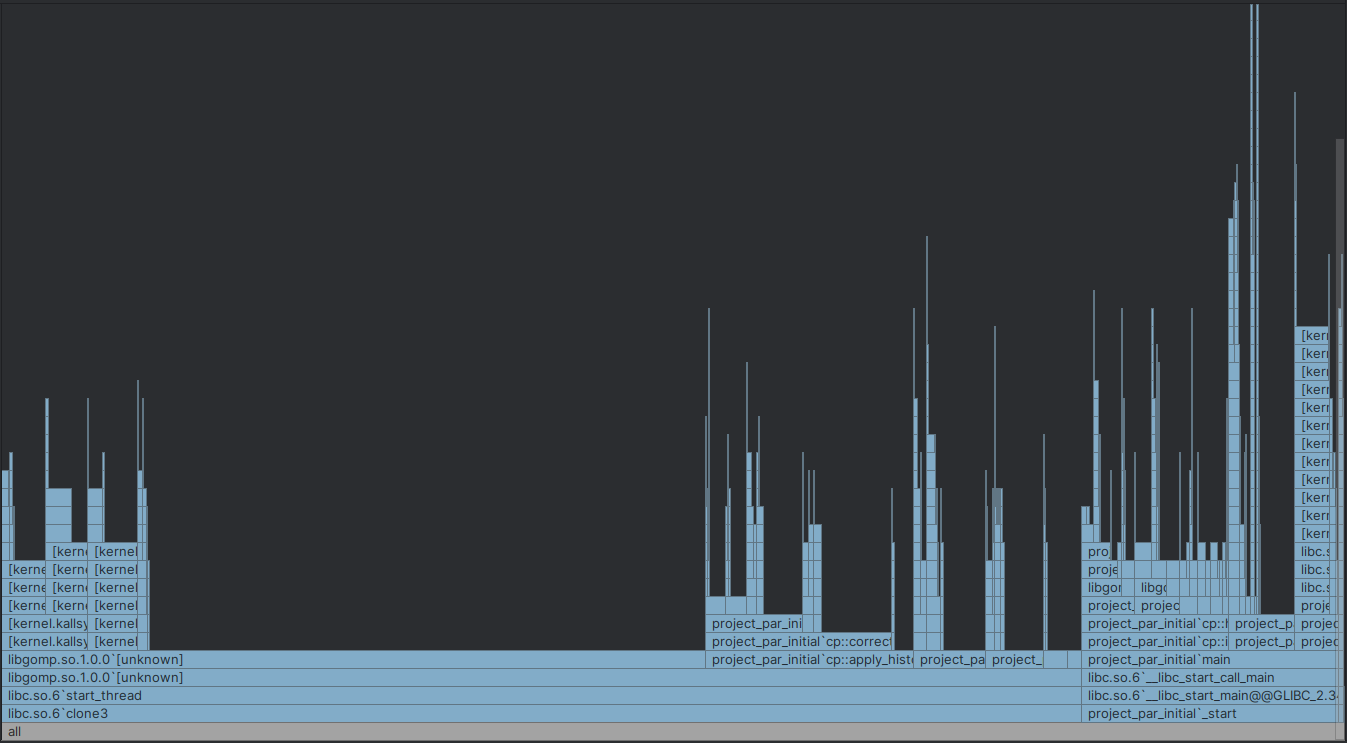
\includegraphics[width=0.5\textwidth]{InitialParallelProfiler.png}
    \caption{CLion Profiler of the First Parallel Version}
\end{figure}

\subsection{Second Parallelization}
\subsubsection{Implementation}
This second implementation is the result of the improvement of the build\textunderscore histogram function. We changed the simple use of "\# pragma omp parallel for" with the use of more complex parallel implementation, by creating local histograms to execute the calculations in parallel and then merge them into the global histogram.
\subsubsection{Performance Analysis}
The performance analysis showed us better performance than the first parallel version. We can also observe that this version showed the best performance when using 8 threads, and not 12.
\begin{figure}[h]
    \centering
    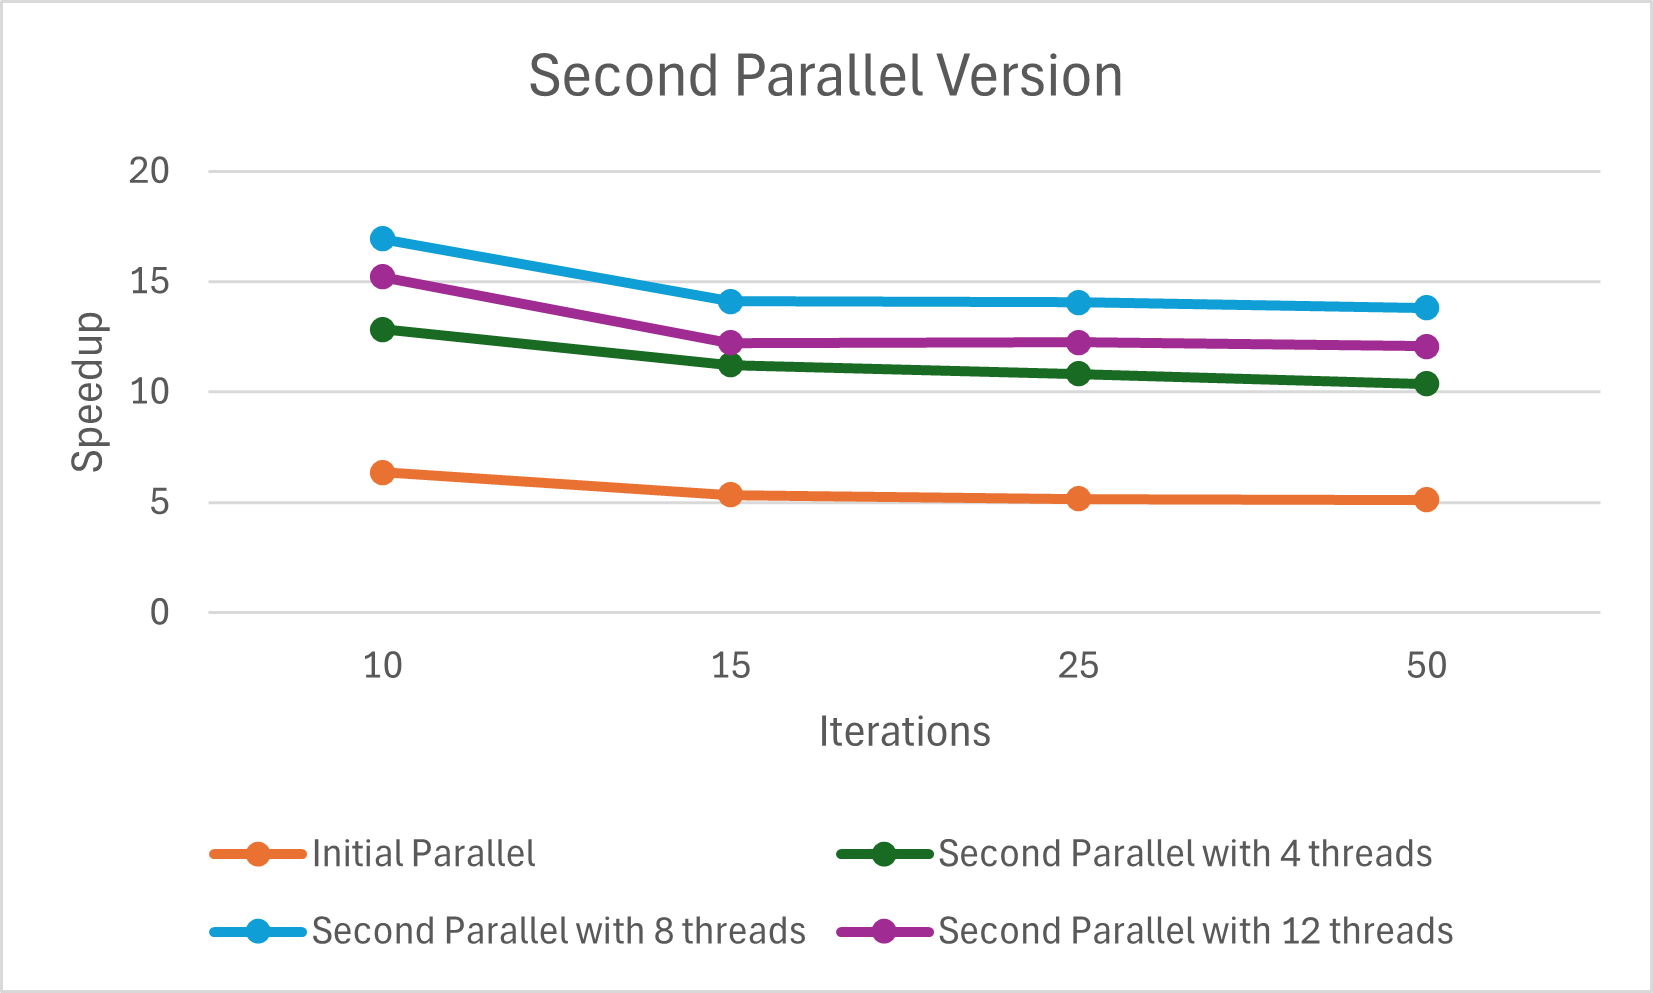
\includegraphics[width=0.5\textwidth]{SecondParallelSpeedup.png}
    \caption{Speedup of the Second VS Initial Parallel versions}
\end{figure}

\subsubsection{Profiler Analysis}
The results of the profiler were pretty similar to the initial parallel version, tho. This is because there was not a significant difference in the solution logic, as the one we will observe with the final parallel version:
\begin{figure}[h]
    \centering
    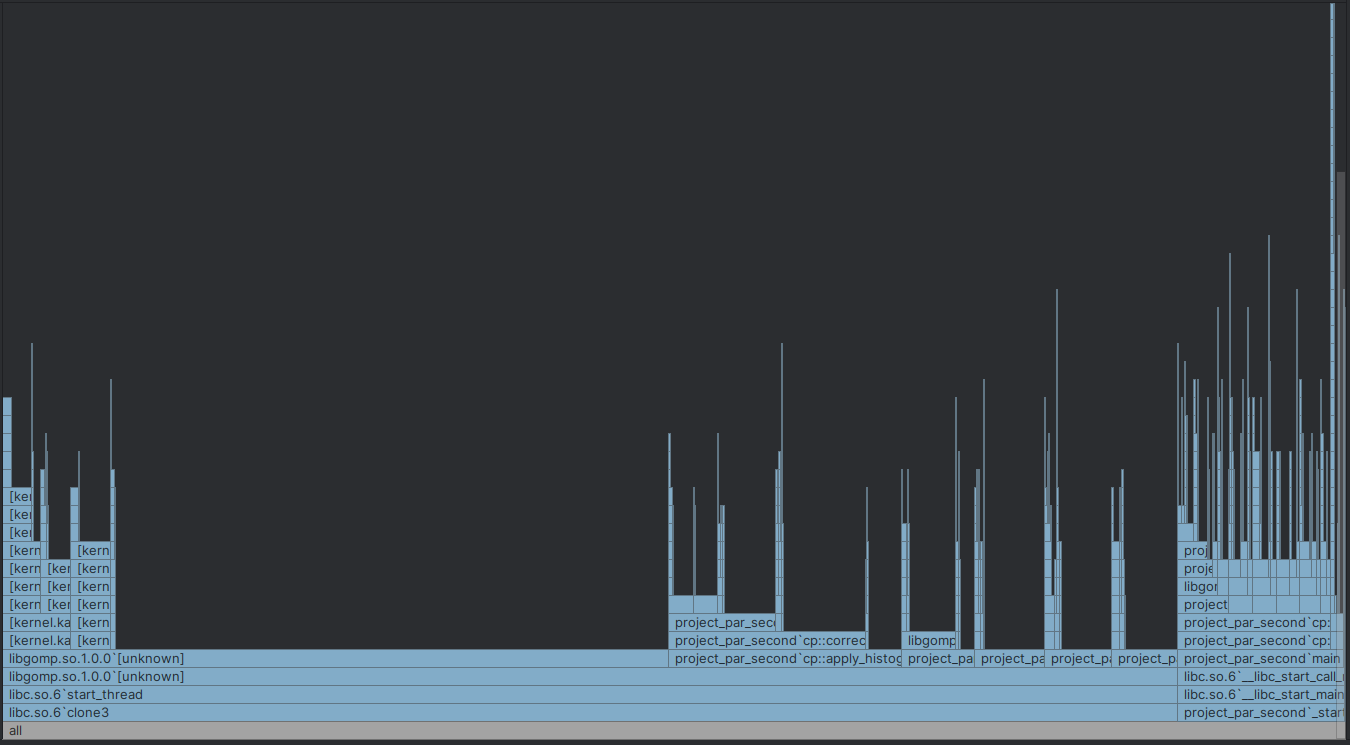
\includegraphics[width=0.5\textwidth]{SecondParallelProfiler.png}
    \caption{CLion Profiller of the Second Parallel Version}
\end{figure}
\subsection{Final Parallelization}
\subsubsection{Implementation}
Our final parallel version consists in joining the following three functions into one:convert\textunderscore to\textunderscore uchar, convert\textunderscore to\textunderscore grayscale and build\textunderscore histogram. This way, instead of having three different loops, we only have one. This also allowed us to remove two arrays of chars(ucchar\textunderscore image and gray\textunderscore image), improving space performance.
\subsubsection{Performance Analysis}
As expected, this was the best performer of all versions. For every different test we made, with images of different sizes and different number of iterations, the final parallel version had always the best performance. In the following graphic we can observe the speedup differences between the second and final versions. This time, we can´t observe a total domination of a specific number of threads. Depending of the image size and the number of iterations, different numbers of threads perform better in different situations.
\begin{figure}[h]
    \centering
    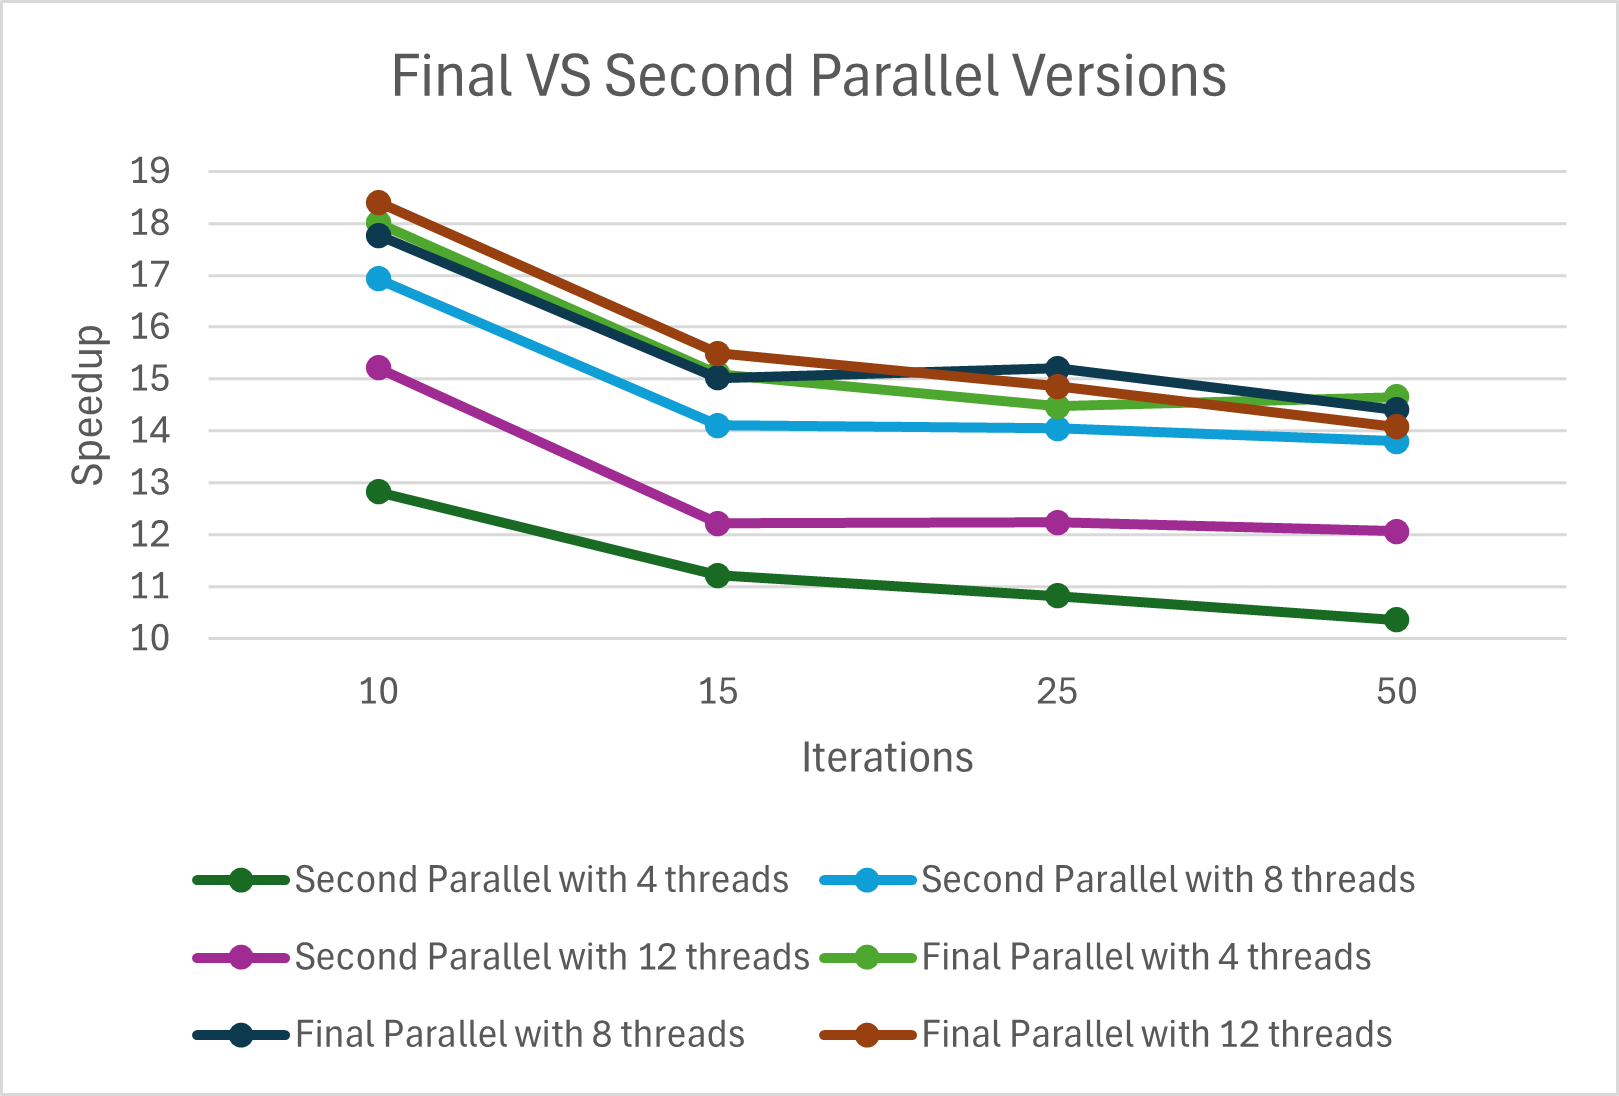
\includegraphics[width=0.5\textwidth]{FinalParallelVersion.png}
    \caption{Speedup of the Final Parallel Version}
\end{figure}

\subsubsection{Profiler Analysis}
This time the profiler analysis shows different result than the previous two versions, since three loops were simplified into one.
\begin{figure}[h]
    \centering
    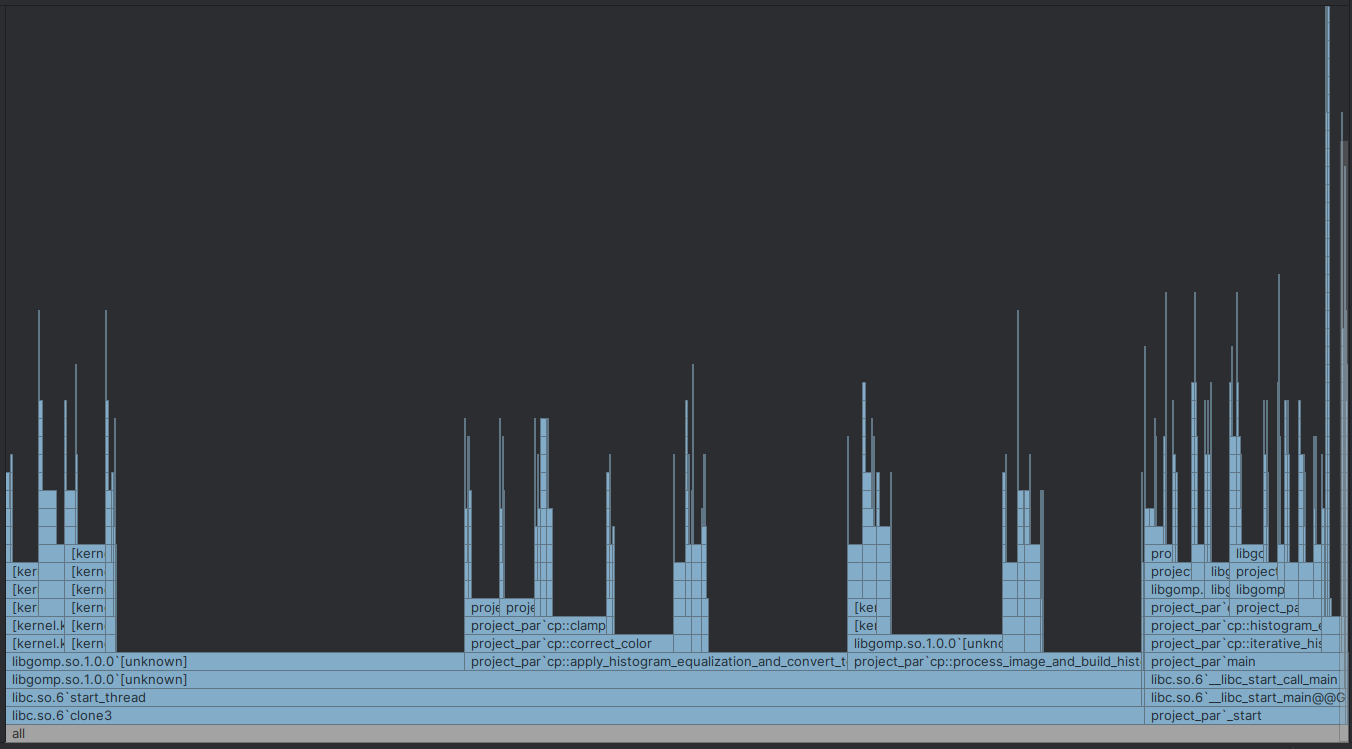
\includegraphics[width=0.5\textwidth]{FinalParallelProfiler.png}
    \caption{Flame Graph of the sequential code}
\end{figure}
\section{Stage 2}
\subsection{Implementation}
The GPU-accelerated version consists of the implementation of the last parallel version (implemented in stage 1), but with the boost of using the GPU.
\subsection{Performance Analysis}
In the following graphic we can observe big improvement in the speedup time. Even with no differences in the implementation logic compared to the final parallel version of stage 1, the use of the GPU brings much more improvement than any other changes made to the initial code. Thus, it is very important to use all available resources when dealing with such problems.
\begin{figure}[h]
    \centering
    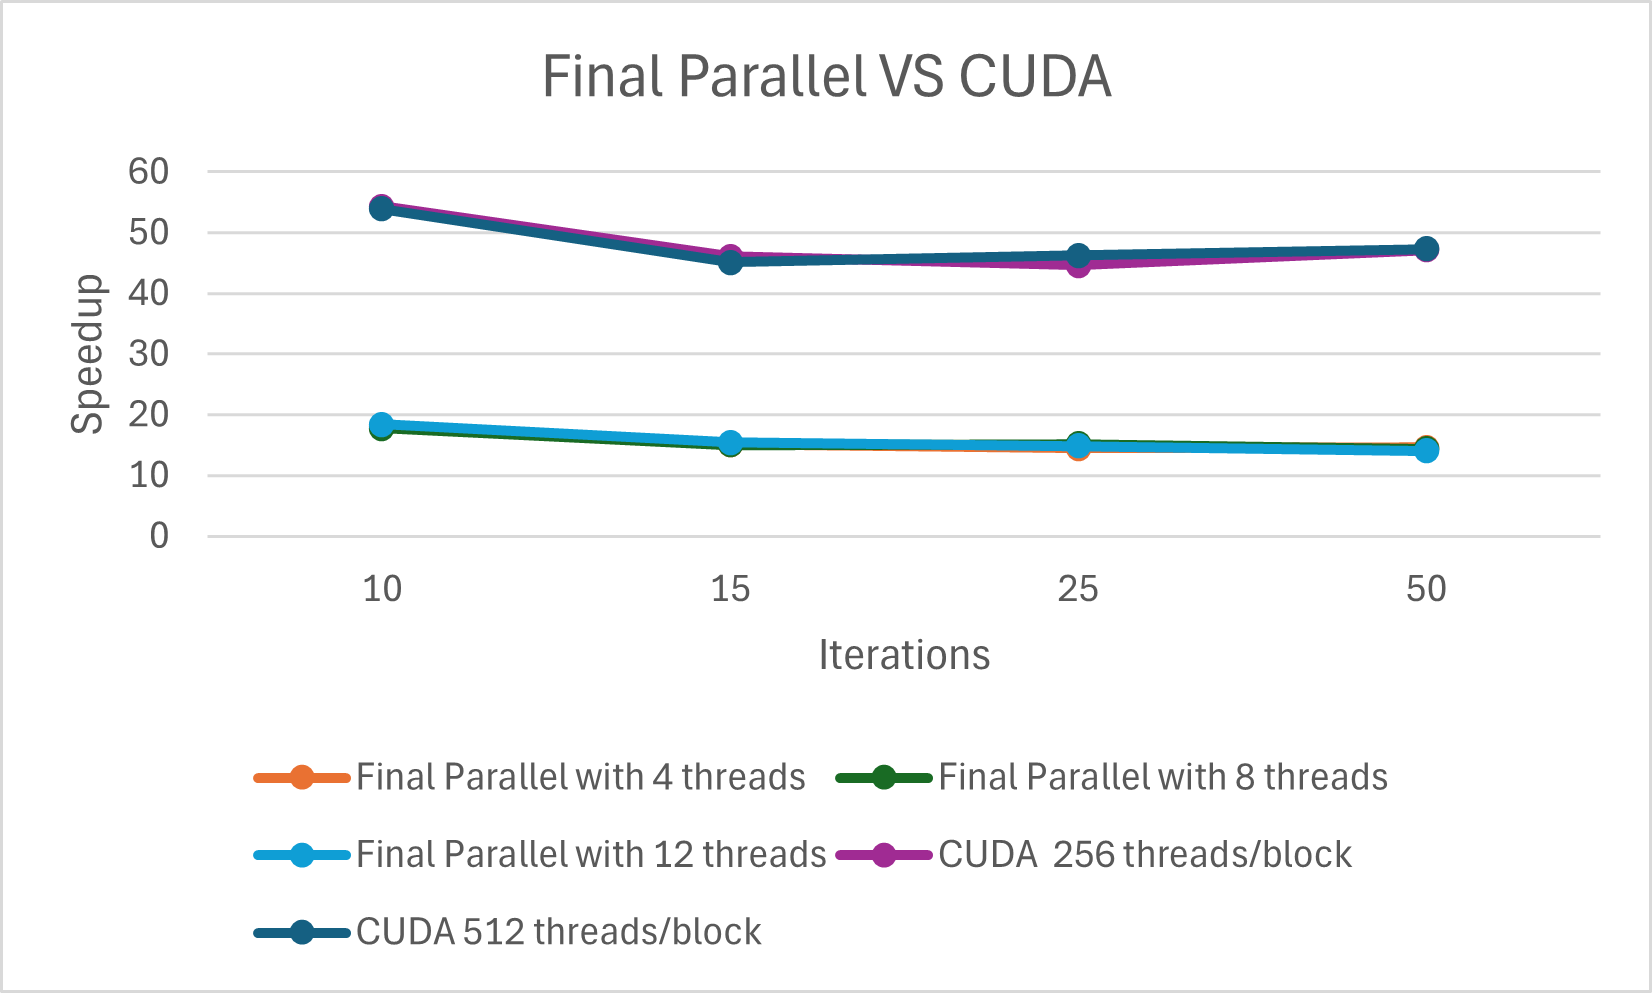
\includegraphics[width=0.5\textwidth]{CUDA.png}
    \caption{Speedup of the Final Parallel Version VS CUDA}
\end{figure}

\section{Overall analysis}
After the implementation of the project and all the tests we run, we conclude the following:
\begin{itemize}
    \item The Final Parallel solution is better than the others in every test case (except for the GPU boost)
    \item More number of threads does not mean better performance. Each case must be evaluated carefully.
    \item Using GPU-accelerated version of the code is way faster. When dealing with such problems, refactoring the code and use OpenMP has its limits in the performance improvement. If we want better performance, we should definitely use the GPU.
\end{itemize}
\section{Individual Contributions}
We had some miscommunication problems (my fault: Martin Magdalinchev), so my colleague ended up by implementing all Stage 1 and Stage 2. When I joined him, he had already done the implementation of Stage 1 and had started the implementation of Stage 2. So I started by preparing the code for testing (separating all parallel versions into their own classes),running some tests and implementing the script. Then my colleague finished Stage 2 and I wrote the report.  


\end{document}
